
%%%%%%%%%%%%%%%%%%%%%%%%%%%%%%%%%%%%%%%%%%%%%%%%%%%%%%%%%%%%%%%%%%% 
%                                                                 %
%                           PREVIOUS WORK                         %
%                                                                 %
%%%%%%%%%%%%%%%%%%%%%%%%%%%%%%%%%%%%%%%%%%%%%%%%%%%%%%%%%%%%%%%%%%% 
 
% \specialhead{PREVIOUS WORK}
\chapter{PREVIOUS WORK}
\label{chapter:previous_work}

In this chapter, I will provide a more in-depth look at previous focus plus context systems and discuss the applicability of these techniques to our application.

\section{Focus Plus Context Visualizations}
\label{section:prev_fc_vis}

One of the earliest systems that tried to tackle the focus plus context problem was the \emph{Perspective Wall} presented by Mackinlay et al. \cite{Mackinlay1991}. This system was integrated with the \emph{Information Visualizer}, a system for visualizing data in 3D. The \emph{Perspective Wall} sought to imitate the nature of the human eye, by having a smooth integration between a focused area and the overall context. This system turns a 2D layout into a 3D wall system which contains
an area of detail surrounded by a distorted region. The \emph{Perspective Wall} had a flat region of high detail with regions surrounding it that were angled to match the field of view of the viewer. An image of the system is seen in Figure~\ref{fig:perspective_wall} showing the areas of magnification and demagnification. The focus of the application was to view information that was structured temporally, such as a filesystem. One of its greatest strengths was that it presented information in an intuitive manner. Unfortunately, while this work showed that such distortion techniques are helpful in facilitating understanding for the users, it is unsuited for our own purposes as this system performs a global distortion of the data and the metaphor does not easily extend to a system with different regions of focus.

\begin{figure}[htp] \centering
    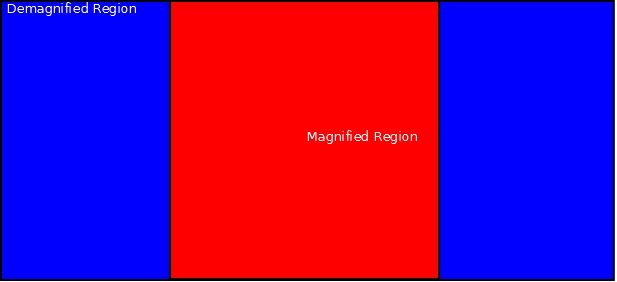
\includegraphics[width=0.45\linewidth]{img/Perspective_Wall.jpg}
    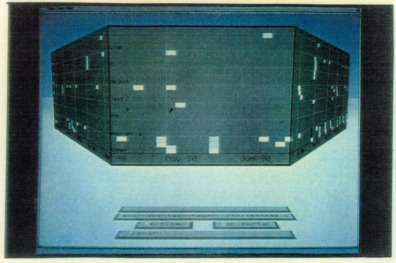
\includegraphics[width=0.45\linewidth]{img/perspective_wall_actual.jpg}
    \caption[Perspective Wall Diagram]{A figure showing the magnified and demagnified regions of the 
        \emph{Perspective Wall} \cite{Mackinlay1991}, and an image of the original system, created by Mackinlay 
        et al.. The blue regions are demagnified and represent the angled areas.}
    \label{fig:perspective_wall}
\end{figure}

Baudisch et al.\ attempted to display focus plus context information through the integration of different hardware into a single logical screen \cite{Baudisch2001}. This screen consists of a low resolution region for context and a high resolution area for detailed information. They achieve similar effects as a fisheye view, but avoid distortion with their hardware. The prototype constructed integrates a LCD screen with a projection screen; a diagram of the system along with an image
of the actual system is seen in Figure~\ref{fig:f_and_c}.  By having two distinct regions of resolution, they are able to maintain the overall
geometry of the displayed images. To achieve this effect, Baudisch et al.\ created a foam core projection screen with a cutout for a flat panel LCD monitor. A large portion of the work performed by Baudisch et al.\ was used for examining this system with different applications. Of particular note is their work with a map application for finding the shortest path between two cities. The display allowed for seeing both the surrounding geography and large highways between the cities, while
allowing the user to also view street-level detail for areas with densely packed information. A single application controls the rendering for both screens. The data is rendered at a resolution that would fill the projection screen if it was also high resolution. A region is clipped to fit the resolution of the LCD monitor, while the overall data is scaled to fit within the projection screen. This solution provides a distortion free visualization, but only has a single area of
higher resolution. Viewing different regions of the data is performed by moving the entire visualization, which is not well suited to interactively viewing different areas simultaneously, but works perfectly fine for a single user. Generating new hardware is also outside of the scope of this thesis, but the studies performed by Baudisch et al.\ provide useful insight. In a small user survey, it was found that the overall responsiveness of the application as well as the ability to see the bigger picture of the work was beneficial for users of the system.

\begin{figure}[htp] \centering
    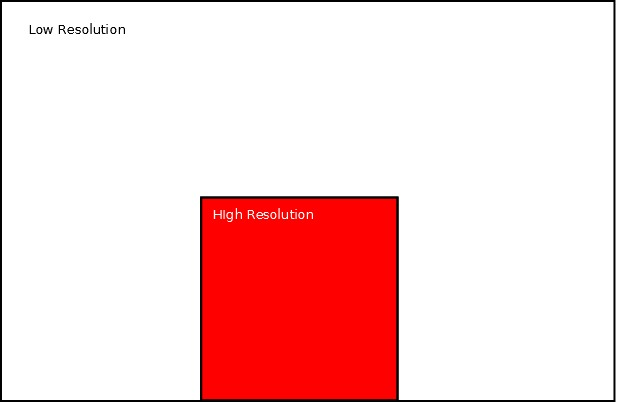
\includegraphics[width=0.45\linewidth]{img/f_and_c.jpg}
    \includegraphics[width=0.45\linewidth]{img/f_and_c_actual.jpg}
    \caption[Focus Plus Context Screen Diagram]{A figure showing the areas of high and low resolution images of 
    the focus plus context \cite{Baudisch2001} system created by Baudisch et al.. The red region is the LCD screen and the white area is the 
    projector screen.}
    \label{fig:f_and_c}
\end{figure}

Following their previous work, a formal study of the benefits of focus plus context displays was performed by Baudisch et al. Three different interfaces were evaluated with a number of different tasks to discover what display techniques were most helpful for completing said tasks \cite{Baudisch2002}. The focus plus context system described previously was compared with a zoom plus pan interface using a single screen and a overview plus detail interface using two monitors. All of the displays had approximately the same number of pixels between them. To further attempt to control for any extra space affecting the result of the experiment, the overview screen in the overview plus detail interface was constrained to the same size as the context of the focus plus context interface, while normally it would show the entirety of whatever dataset is being observed. There were two different types of tasks asked of the participants, the first was a static view where the users had to either
verify connections on a circuit board or find the closest hotel to a given point, and the second was a dynamic application where users were tasked with avoiding rocks and nails in a simple simulation. It was hypothesized and discovered that the focus plus context interface was the most helpful for performing both types of tasks. These results are promising for the infrastructure visualization, it suggests that a view providing a seamless integration between global and local data is most helpful in performing tasks which require both types of data. 

Gansner et al.\ describe a method for rendering sets of data with millions of nodes \cite{Gansner2005}. Their method, which they name ``Topological Fisheye'', follows the general principle given by Furnas et al.\ in  by having a detailed region around a focus with less information in other areas \cite{Furnas1986}. To reduce the amount of data in areas
out of focus, they create approximations of the original graph. When an area comes into focus, a hybrid graph is constructed by combining the various different approximations based on the distance from the focal point. To simplify the graph, they generate a proximity graph using either Delauney triangulation or a relative neighborhood graph and combine the results with the original edges of the graph to form a candidate set S. This set is then filtered by maximizing a weighted sum
of various measurements of the two points to be collapsed. The methods described in this construction are definitely applicable to future versions of the infrastructure visualization. As our data set grows, we may need to first simplify our graph data to filter out less important nodes. This filtered data could then be further transformed by a geometric transformation. A pure application of this would not adequately modify the underlying satellite images of our graph network.

\section{Geometric Transformations}
\label{section:prev_geometric_transformations}

As mentioned in Section~\ref{section:intro_fac}, the generalized fisheye view was described by Furnas in 1986 \cite{Furnas1986}. This method was later reworked in 1992 by Sarkar and Brown, who produced a method for performing geometric transformations to visually distort graphs and maps. This method changes the position, size, and level of detail based on the distance between the original object and the point of focus. An important distinction between this work and the generalized fisheye view is that the latter has objects either completely visible or not present at all, while this graphical method allows for a continuum \cite{Sarkar1992}.

Vertices are first positioned away from the focus via a transformation function. Given a vertex's original position, $P_{norm}$, the position of the focus, $P_{focus}$, and the max distance a vertex can move, $D_{max}$, the resulting fisheye position, $P_{feye}$ can be calculated.

\begin{equation}
    \label{eq:sarkar_fisheye} 
    P_{feye} = G(P_{norm})D_{max} + P_{focus}
\end{equation}

$G(P_{norm})$ is a monotonically increasing function that is continuous over the range $0 \leq x \leq 1$ with $G(0) = 0$ and $G(1) = 1$. 

\begin{equation}
    \label{eq:g_sarkar} 
    G(P_{norm}) = \frac{d + 1}{d + \frac{D_{max}}{D_{norm}}}
\end{equation}

In the above equation, $D_{norm}$ is the distance from the original point to the focal point, and $d$ is a distortion factor.

This general equation provides the basis for the transformations discussed later in Section~\ref{chapter:magnification}. The resulting new point of the transformation we apply to points should be based on the original location for the vertex and the location for a focal point. While Equation~\ref{eq:sarkar_fisheye} is helpful in creating a solution to our visualization problem, the distortion factor does not cleanly map to a degree of magnification. This distortion is helpful
for visualizing purely graph based data, but does not directly apply to magnification of images. When viewing a satellite image, being able to modify the magnification to any amount is important, as more detail is shown through this process. Graph based data does not need this type of magnification, as it only further increases the distance between elements.

Similar geometric transformations are discussed  by Kadmon and Shlomi\ for the distortion of maps with multiple focal regions \cite{Kadmon1978}. A similar basic function is given for transforming the scale of the map at a given point, \emph{P}, with a original scale $S_0$, the original distance from $P$ to the focus, $R$, and a distance function $f(R)$.

\begin{equation}
    \label{eq:kadmon_polyfocal} 
    S = S_0 + S_0 f(R)
\end{equation}

Unlike the equations created by Sarkar and Brown, Equation~\ref{eq:kadmon_polyfocal} is defined over the entire input. It exhibits similar behaviors in that the function $f(R)$ is chosen to cause $S$ to decrease as $R$ increases. Kadmon and Shlomi give the following general equation for $f(R)$.

\begin{equation}
    \label{eq:f_kadmon}
    f(R) = \frac{A}{1 + CR^2}
\end{equation}

The constant factors $A$ and $C$ represent the power of the focus and the rate of change, respectively. This pair of equations has a similar problem of constants which result in unclear transformations for the implementation. Being able to modify the scale to set amounts allows users to switch between views consistently and avoid confusion that would occur if the scale factor was not discrete steps. An additionally helpful insight from is that points which are affected by multiple
foci at the same time are affected by the sum of the individual foci \cite{Kadmon1978}. This insight is useful for the implementation of our own magnification functions when dealing with multiple areas of magnification.

The idea of magnification transformations is explored further by Keahey and Robertson. They propose the idea of combining linear and non-linear transformation functions to take advantage of the strengths of both. Linear functions are often desirable due to the fact that they perform zooming without introducing distortion into the system. This region of linear zoom can be important when trying to read text or other data that is sensitive to distortion. The non-linear region trades
distortion for the ability to fit more data in a smaller area. The resulting piecewise transformation allows a user to view a region in high detail while still retaining the context of the surrounding data. The application of this combination is seen in Figure~\ref{fig:regions_diagram}, which illustrates a region of linear magnification surrounded by a region of non-linear magnification

\begin{figure}[htp] \centering
    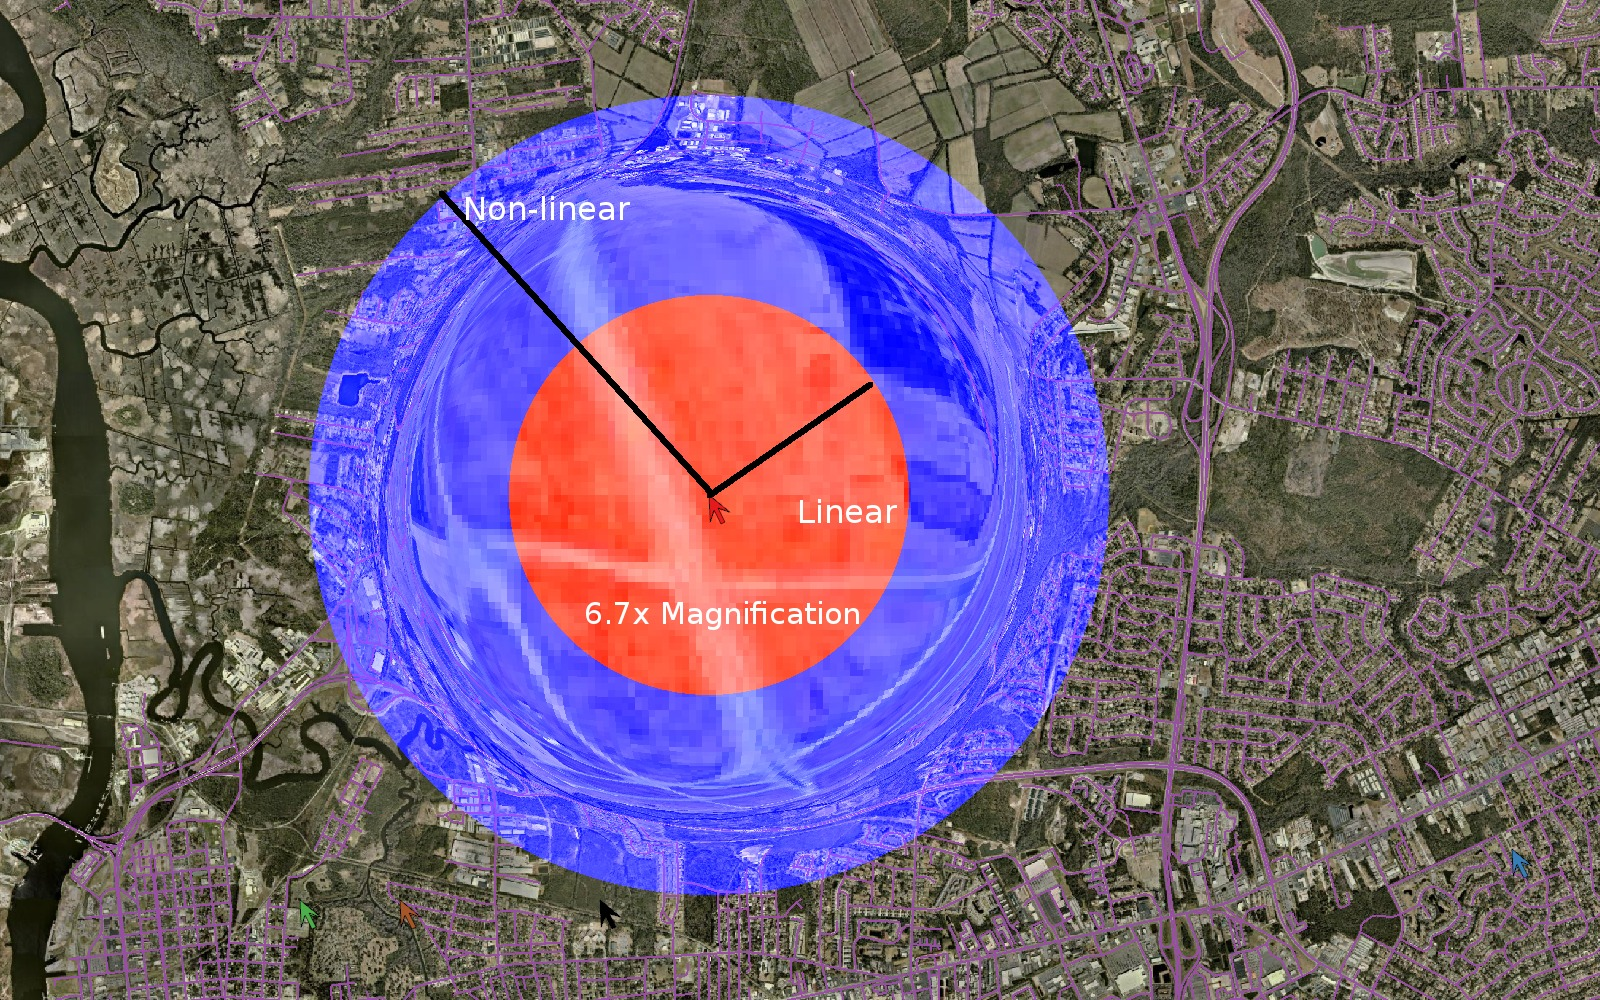
\includegraphics[width=0.8\linewidth]{img/regions_diagram.jpg}
    \caption[Combined Linear and Non-linear Magnification Regions]{An image of our infrastructure visualization magnification regions. The blue area is the non-linear magnification and the red region is the linear magnification. Note that despite being distorted, the roads in the image are still connected in both regions, allowing the user to trace a continuous path.}
    \label{fig:regions_diagram}
\end{figure}

Keahey and Robertson also note that performing such transformations on different domains has different requirements. When manipulating graph networks, the overall adjacency of nodes and edges is maintained for most transformations, linear or non-linear. Visual data requires more focus on the boundaries between the different transformation functions, as the boundary regions are especially susceptible to visual errors if they are not C0 continuous. An example image of a
magnification function that is not C0 continuous is seen in Figure~\ref{fig:non_continuous}. This resulting magnification includes a loss of data due to the discontinuity. These concerns are directly
applicable to designing a solution, as our data is stored in both a graph network and a series of satellite images. 

\begin{figure}[htp] \centering
    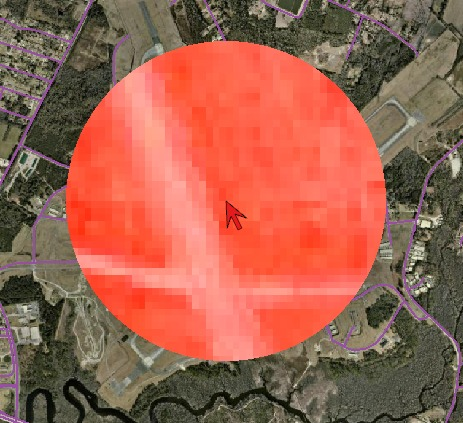
\includegraphics[width=0.3\linewidth]{img/non_continuous.jpg}
    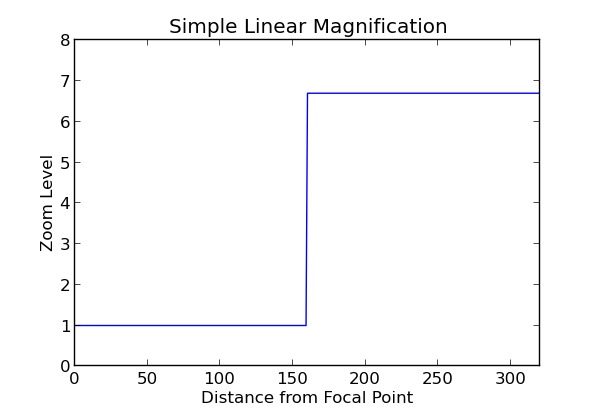
\includegraphics[width=0.6\linewidth]{img/discontinuity_graph.jpg}
    \caption[Loss of Visual Data]{The magnification function for this transformation is not C0 continuous, and as such, causes a loss of data and discontinuities of geographic data.}
    \label{fig:non_continuous}
\end{figure}

In addition to discussing the relevant concerns of combining transformation functions, Keahey and Robertson describe a few methods for combining regions of magnification. Of particular note is his proposal for weighted averaging that simply transforms a point by all nearby functions and calculates weights as the inverse of the distance between the center of magnification and the original point. This method does not obscure data, and is simple to implement for our purposes

In this new paper, Keahey and Robertson generalize the non-linear magnification problem by removing the concept of foci \cite{Keahey1997}. They make a distinction between transformation and magnification, where the former indicates the distortion of the space, with the magnification function being the derivative of the transformation function. By generalizing the problem to a scalar field, we can derive the magnification of a particular element based on its own properties. Given a particular magnification mesh, computing a corresponding transformation grid is difficult, as it involves trying to convert a single magnification value into a two coordinate system. The solution presented uses an iterative method to approximate a numerical solution. The work done in is well suited to the task at hand for our data when either the satellite images or graph network are displayed
independently. However, we still need to create our own magnification functions to modify the underlying scalar field and create a region of linear zoom. This method simply removes the need for thinking about the magnification problem with regards to focal points. 

Keahey later generalizes the overall focus plus context problem into a detail plus context problem \cite{Keahey1998}. Up to this point, most focus context systems create focus by enlarging specific regions while compressing other regions. This does not inherently produce more detail within this region, as it simply makes the existing data easier to distinguish. He proposes a few different methods of adding detail to such regions like displaying different view levels. By
showing different view levels, the amount of information displayed in a region changes, as the original non-linear transformation merely causes a change in terms of size and shape. He mentions that this process could be used for map based data, and this technique is definitely helpful for future work (Chapter~\ref{chapter:future_work}).

In contrast to the fisheye visualizations of data presented by Kadmon and Shlomi, Sarkar and Brown, and Keahey and Robertson,  Elmqvist et al.\ present a method for folding space to achieve a focus plus context view \cite{Kadmon1978} \cite{Sarkar1992} \cite{Keahey1996} \cite{Elmqvist2010}. The other techniques present a visualization that is visually similar to a fisheye lens, focusing more on having a lot of global data. This method contextually folds 2D data into 3D such that
the only regions displayed are areas within focus. This devotes most of the screen space to the focal points at the cost of being able to see most of the global data. Where other techniques that utilize focus plus context expand the region around focal points, the system
created by Elmqvist et al.\, M\'{e}lange, compresses the
unimportant areas of the display. A diagram of this system is seen in Figure~\ref{fig:melange}, notice that the red region, corresponding to the magnified areas, take up the majority of the display. Relative distance between focal points within the distorted region is represented by a number of folds, each indicating a complete screen distance. While this method produces interesting results, it is important in our visualization to have a majority of the information undistorted. M\'{e}lange focuses on showing as much detail around the focal points as possible, but the goals for a visualization of our system are to show a smaller area of increased focus while maintaining as much context as possible.

\begin{figure}[htp] \centering
    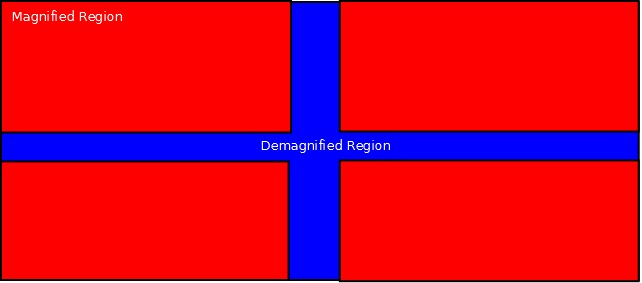
\includegraphics[width=0.45\linewidth]{img/Melange.jpg}
    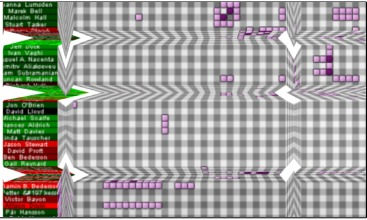
\includegraphics[width=0.45\linewidth]{img/melange_actual.jpg}
    \caption[M\'{e}lange Diagram]{An image comparing magnified and demagnified regions of the M\'{e}lange system 
    \cite{Elmqvist2010}, developed by Elmqvist et al.\ as well as the system applied to a visualization of an   
    adjacency diagram.}
    \label{fig:melange}
\end{figure}

B\"{o}ttger et al.\ present a method for manipulating a distorted city map to highlight specific areas of interest in \cite{Bottger2008}. The motivation for this system was the combination of geographic data and a stylized subway network to display more information around areas on the stylized network diagram. They introduce a concept called \emph{Warping Zoom}. Given a set of control points, they create a mapping function which moves any number of control points to other positions.
These individual control points correspond to the different subway stops and routes on the original mapping and are moved to positions to form the stylized network. While this method would allow for the separation of clustered data within our visualization by warping the overall data, it does not provide a solution for viewing the satellite data at a higher level of detail, nor does it perform an easily classifiable magnification function. To perform a magnification of a region of
satellite images, the system would have to define multiple control points and their resulting position. This is essentially performing the same transformation as a simple magnification function, but only focuses on manipulating a few points. 

\section{Summary}
\label{section:PREVIOUS_WORK_SUMMARY}

This chapter provided an overview of works which attempt to use a focus plus context visualization. I discussed a variety of applications which focused on utilizing some sort of focus plus context solution to solve their visualization issues. Finally, applications and research which concerned geometric distortions of data were summarized with respect to our goals. The following chapter discusses the changes performed to our visualization to improve performance and allow for implementation of our magnification function.
